% Copyright 2019 by Till Tantau
%
% This file may be distributed and/or modified
%
% 1. under the LaTeX Project Public License and/or
% 2. under the GNU Free Documentation License.
%
% See the file doc/generic/pgf/licenses/LICENSE for more details.


\section{Syntax for Path Specifications\\路径规范的语法}
\label{section-paths}

A \emph{path} is a series of straight and curved line segments. It is specified
following a |\path| command and the specification must follow a special syntax,
which is described in the subsections of the present section.

\emph{路径}是一系列直线和曲线线段。它在 |\path| 命令后面指定,并且规范必须遵循特定的语法,该语法在本节的子段中描述。

\begin{command}{\path\meta{specification}|;|}
    This command is available only inside a |{tikzpicture}| environment.

    此命令仅在 |{tikzpicture}| 环境内可用。

    The \meta{specification} is a long stream of \emph{path operations}. Most
    of these path operations tell \tikzname\ how the path is built. For
    example, when you write |--(0,0)|, you use a \emph{line-to operation} and
    it means ``continue the path from wherever you are to the origin''.

    \meta{规范} 是一长串的\emph{路径操作}。大多数路径操作告诉 \tikzname\ 如何构建路径。例如,当您写 |--(0,0)| 时,您使用了一种\emph{线到操作},它表示``从当前位置继续路径到原点''。

    At any point where \tikzname\ expects a path operation, you can also give
    some graphic options, which is a list of options in brackets, such as
    |[rounded corners]|. These options can have different effects:
    
    在任何期望路径操作的位置上,您也可以给出一些图形选项,即方括号中的选项列表,例如 |[rounded corners]|。这些选项可以具有不同的效果:
    %
    \begin{enumerate}
        \item Some options take ``immediate'' effect and apply to all
            subsequent path operations on the path. For example, the
            |rounded corners| option will round all following corners, but not
            the corners ``before'' and if the |sharp corners| is given later on
            the path (in a new set of brackets), the rounding effect will end.
            %

            某些选项立即生效,并适用于路径上的所有后续路径操作。例如,|rounded corners| 选项将使后续的所有角都变圆,但不会影响``之前''的角,如果在路径中稍后(在新的一对方括号中)给出 |sharp corners|,则圆角效果将结束。
\begin{codeexample}[]
\tikz \draw (0,0) -- (1,1)
           [rounded corners] -- (2,0) -- (3,1)
           [sharp corners] -- (3,0) -- (2,1);
\end{codeexample}
            %
            Another example are the transformation options, which also apply
            only to subsequent coordinates.

            另一个例子是变换选项,它们也仅适用于后续的坐标。

        \item The options that have immediate effect can be ``scoped'' by
            putting part of a path in curly braces. For example, the above
            example could also be written as follows:

            立即生效的选项可以通过将路径的一部分放在花括号中进行作用域限定''。例如,上面的示例也可以写成如下形式: 
            %
\begin{codeexample}[]
\tikz \draw (0,0) -- (1,1)
           {[rounded corners] -- (2,0) -- (3,1)}
           -- (3,0) -- (2,1);
\end{codeexample}
            %
        \item Some options only apply to the path as a whole. For example,
            the |color=| option for determining the color used for, say,
            drawing the path always applies to all parts of the path. If
            several different colors are given for different parts of the
            path, only the last one (on the outermost scope) ``wins'':
            %

            某些选项仅适用于整个路径。例如,|color=| 选项用于确定用于绘制路径的颜色,始终适用于路径的所有部分。如果为路径的不同部分给出了多种不同的颜色,只有外层作用域中的最后一个颜色生效'':
\begin{codeexample}[]
\tikz \draw (0,0) -- (1,1)
           [color=red] -- (2,0) -- (3,1)
           [color=blue] -- (3,0) -- (2,1);
\end{codeexample}

            Most options are of this type. In the above example, we would
            have had to ``split up'' the path into several |\path| commands:
            
            大多数选项都是此类型。在上面的示例中,我们必须将路径``拆分''为几个 |\path| 命令:
\begin{codeexample}[]
\tikz{\draw (0,0) -- (1,1);
      \draw [color=red] (1,1) -- (2,0) -- (3,1);
      \draw [color=blue] (3,1) -- (3,0) -- (2,1);}
\end{codeexample}
    \end{enumerate}

    By default, the |\path| command does ``nothing'' with the path, it just
    ``throws it away''. Thus, if you write |\path(0,0)--(1,1);|, nothing is
    drawn in your picture. The only effect is that the area occupied by the
    picture is (possibly) enlarged so that the path fits inside the area. To
    actually ``do'' something with the path, an option like |draw| or |fill|
    must be given somewhere on the path. Commands like |\draw| do this
    implicitly.

    默认情况下,|\path| 命令对路径不进行任何操作,只是将其``丢弃''。因此,如果您写 |\path(0,0)--(1,1);|,则不会在您的图片中绘制任何内容。唯一的效果是图片所占用的区域(可能)扩大,以便路径适合该区域。要对路径进行实际``操作'',必须在路径的某个位置上给出像 |draw| 或 |fill| 这样的选项。像|\draw| 这样的命令会隐式执行此操作。

    Finally, it is also possible to give \emph{node specifications} on a path.
    Such specifications can come at different locations, but they are always
    allowed when a normal path operation could follow. A node specification
    starts with |node|. Basically, the effect is to typeset the node's text as
    normal \TeX\ text and to place it at the ``current location'' on the path.
    The details are explained in Section~\ref{section-nodes}.

    最后,还可以在路径上给出\emph{节点规范}。这样的规范可以出现在不同的位置,但只要可以跟随普通路径操作,就始终允许它们。节点规范以 |node| 开头。基本上,效果是将节点的文本作为普通的 \TeX\ 文本排版,并将其放置在路径的``当前位置''上。详细信息请参见第~\ref{section-nodes} 节。

    Note, however, that the nodes are \emph{not} part of the path in any way.
    Rather, after everything has been done with the path what is specified by
    the path options (like filling and drawing the path due to a |fill| and a
    |draw| option somewhere in the \meta{specification}), the nodes are added
    in a post-processing step.

    但请注意,节点在任何方式上都\emph{不是}路径的一部分。相反,在按照路径选项的规范执行路径的所有操作后(例如由于在 \meta{规范} 中的某个位置给出了 |fill| 和 |draw| 选项而绘制路径),节点将在后处理步骤中添加。

    \emph{Note:} When scanning for path operations \tikzname\ expands tokens
    looking for valid path operations. This however implies that these tokens
    has to be fully expandable up to the point where it results in a valid path
    operation.

    \emph{注意:}在扫描路径操作时,\tikzname\ 展开标记以查找有效的路径操作。然而,这意味着这些标记必须在完全可展开的情况下扩展,直到结果形成有效的路径操作为止。
\end{command}

\begin{key}{/tikz/name=\meta{path name}}
    Assigns a name to the path for reference (specifically, for reference
    in animations; for reference in intersections, use the |name path|
    command, which has a different purpose, see the |intersections| library
    for details). Since the name is a ``high-level'' name (drivers never
    know of it), you can use spaces, number, letters, or whatever you like
    when naming a path, but the name may \emph{not} contain any punctuation
    like a dot, a comma, or a colon.

    为路径分配一个名称以供引用(具体来说,用于动画中的引用;要引用交点,请使用具有不同目的的 |name path| 命令,请参见 |intersections| 库以获取详细信息)。由于名称是``高级''名称(驱动程序不知道它),因此在为路径命名时可以使用空格、数字、字母或其他任何喜欢的字符,但名称\emph{不能}包含任何标点符号,如点、逗号或冒号。
\end{key}

The following style influences scopes:


以下样式影响作用域:

%
\begin{stylekey}{/tikz/every path (initially \normalfont empty)}
    This style is installed at the beginning of every path. This can be
    useful for (temporarily) adding, say, the |draw| option to everything
    in a scope.
    
    此样式在每个路径的开头处安装。这对于(临时)将诸如 |draw| 选项添加到作用域中的所有内容非常有用。%
\begin{codeexample}[]

\begin{tikzpicture}
  [fill=yellow!80!black,      % only sets the color
   every path/.style={draw}]  % all paths are drawn
  \fill  (0,0) rectangle +(1,1);
  \shade (2,0) rectangle +(1,1);
\end{tikzpicture}
\end{codeexample}
    %
\end{stylekey}

\begin{key}{/tikz/insert path=\meta{path}}
    This key can be used inside an option to add something to the current path.
    This is mostly useful for defining styles that create graphic contents.
    This option should be used with care, for instance it should not be used as
    an argument of, say, a |node|. In the following example, we use a style to
    add little circles to a path.
    %

    此键可在选项内部使用,以将某些内容添加到当前路径。这在定义创建图形内容的样式时非常有用。但是,应谨慎使用此选项,例如不应将其用作 |node| 的参数。在以下示例中,我们使用一个样式向路径添加小圆圈。
\begin{codeexample}[]
\tikz [c/.style={insert path={circle[radius=2pt]}}]
  \draw (0,0) -- (1,1) [c] -- (3,2) [c];
\end{codeexample}
    %
     The effect is the same as of
    |(0,0) -- (1,1) circle[radius=2pt] -- (3,2) circle[radius=2pt]|.

    效果与 |(0,0) -- (1,1) circle[radius=2pt] -- (3,2) circle[radius=2pt]| 相同。
\end{key}

The following options are for experts only:

以下选项仅供专家使用:



\begin{key}{/tikz/append after command=\meta{path}}
    Some of the path commands described in the following sections take optional
    arguments. For these commands, when you use this key inside these options,
    the \meta{path} will be inserted \emph{after} the path command is done. For
    instance, when you give this command in the option list of a node, the
    \meta{path} will be added after the node. This is used by, for instance,
    the |label| option to allow you to specify a label in the option list of a
    node, but have this |label| cause a node to be added after another node.
    %

    下面几节中描述的某些路径命令接受可选参数。对于这些命令,当你在这些选项内部使用此键时,\meta{path} 将被插入在路径命令完成之后。例如,当你在节点的选项列表中给出此命令时,\meta{path} 将添加在节点之后。这在 |label| 选项中使用,允许你在节点的选项列表中指定一个标签,但是在另一个节点之后添加此 |label|。

\begin{codeexample}[]
\tikz \draw node [append after command={(foo)--(1,1)},draw] (foo){foo};
\end{codeexample}
    %
    If this key is called multiple times, the effects accumulate, that is, all
    of the paths are added in the order to keys were found.

    如果多次调用此键,则效果会累积,即以找到键的顺序添加所有路径。

\end{key}

\begin{key}{/tikz/prefix after command=\meta{path}}
    Works like |append after command|, only the accumulation order is inverse:
    The \meta{path} is added before any earlier paths added using either
    |append after command| or |prefix after command|.

    类似于 |append after command|,只是累积顺序相反:\meta{path} 会在使用 |append after command| 或 |prefix after command| 添加的早期路径之前添加。

\end{key}


\subsection{The Move-To Operation\\移动操作}

The perhaps simplest operation is the move-to operation, which is specified by
just giving a coordinate where a path operation is expected.

可能最简单的操作是移动操作,它通过指定一个坐标来指定。

\begin{pathoperation}[noindex]{}{\meta{coordinate}}
        \index{empty@\protect\meta{empty} path operation}%
        \index{Path operations!empty@\protect\texttt{\meta{empty}}}%
    The move-to operation normally starts a path at a certain point. This does
    not cause a line segment to be created, but it specifies the starting point
    of the next segment. If a path is already under construction, that is, if
    several segments have already been created, a move-to operation will start
    a new part of the path that is not connected to any of the previous
    segments.
    %

    移动操作通常从某个点开始一个路径。这不会创建线段,但它指定了下一个线段的起点。如果路径已经在构建中,也就是已经创建了几个线段,那么移动操作将开始一个新的路径部分,不连接到任何先前的线段。

\begin{codeexample}[]
\begin{tikzpicture}
  \draw (0,0) --(2,0) (0,1) --(2,1);
\end{tikzpicture}
\end{codeexample}

    In the specification |(0,0) --(2,0) (0,1) --(2,1)| two move-to operations
    are specified: |(0,0)| and |(0,1)|. The other two operations, namely
    |--(2,0)| and |--(2,1)| are line-to operations, described next.

    在规范 |(0,0) --(2,0) (0,1) --(2,1)| 中,指定了两个移动操作:|(0,0)| 和 |(0,1)|。其他两个操作,即 |--(2,0)| 和 |--(2,1)| 是线段操作,稍稍后解释。

\end{pathoperation}

There is special coordinate called |current subpath start| that is always at
the position of the last move-to operation on the current path.
%

有一个特殊的坐标称为 |current subpath start|,它始终位于当前路径上最后一个移动操作的位置。

\begin{codeexample}[]
\tikz [line width=2mm]
  \draw (0,0) -- (1,0) -- (1,1)
        -- (0,1) -- (current subpath start);
\end{codeexample}

Note how in the above example the path is not closed (as |--cycle| would do).
Rather, the line just starts and ends at the origin without being a closed
path.

请注意,在上面的示例中,路径不是封闭的(就像 |--cycle| 一样)。相反,线只是从原点开始并结束,而不形成封闭路径。


\subsection{The Line-To Operation\\线段操作}

\subsubsection{Straight Lines\\直线}

\begin{pathoperation}{--}{\meta{coordinate or cycle}}
    The line-to operation extends the current path from the current point in a
    straight line to the given \meta{coordinate} (the ``or cycle'' part is
    explained in a moment). The ``current point'' is the endpoint of the
    previous drawing operation or the point specified by a prior move-to
    operation.

    线段操作将当前路径从当前点沿直线延伸到给定的 \meta{坐标}(稍后将解释“或循环”部分)。“当前点”是前一个绘制操作的终点,或者是先前的移动到操作指定的点。


    When a line-to operation is used and some path segment has just been
    constructed, for example by another line-to operation, the two line
    segments become joined. This means that if they are drawn, the point where
    they meet is ``joined'' smoothly. To appreciate the difference, consider
    the following two examples: In the left example, the path consists of two
    path segments that are not joined, but they happen to share a point, while
    in the right example a smooth join is shown.
    %

    当使用线段操作并且刚刚构建了某个路径段,例如通过另一个线段操作,这两个线段将连接在一起。这意味着,如果绘制它们,它们相交的点将被平滑地“连接”起来。为了了解区别,请考虑以下两个示例:在左侧示例中,路径由两个未连接的路径段组成,但它们恰好共享一个点,而在右侧示例中显示了平滑连接。


\begin{codeexample}[]

\begin{tikzpicture}[line width=10pt]
  \draw (0,0) --(1,1)  (1,1) --(2,0);
  \draw (3,0) -- (4,1) -- (5,0);
  \useasboundingbox (0,1.5); % make bounding box higher
\end{tikzpicture}
\end{codeexample}

    Instead of a coordinate following the two minus signs, you can also use the
    text |cycle|. This causes the straight line from the current point to go to
    the last point specified by a move-to operation. Note that this need not be
    the beginning of the path. Furthermore, a smooth join is created between
    the first segment created after the last move-to operation and the straight
    line appended by the cycle operation.

    在两个减号后面不是使用坐标,您还可以使用文本 |cycle|。这会导致从当前点到由移动到操作指定的最后一个点的直线。请注意,这不一定是路径的起点。此外,在最后一个移动到操作之后创建的第一个路径段和循环操作附加的直线之间创建平滑连接。



    Consider the following example. In the left example, two triangles are
    created using three straight lines, but they are not joined at the ends. In
    the second example cycle operations are used.
    
    考虑以下示例。在左侧示例中,使用三条直线创建了两个三角形,但它们的末端未连接。在第二个示例中使用了循环操作。


\begin{codeexample}[]

\begin{tikzpicture}[line width=10pt]
  \draw (0,0) -- (1,1) -- (1,0) -- (0,0) (2,0) -- (3,1) -- (3,0) -- (2,0);
  \draw (5,0) -- (6,1) -- (6,0) -- cycle (7,0) -- (8,1) -- (8,0) -- cycle;
  \useasboundingbox (0,1.5); % make bounding box higher
\end{tikzpicture}
\end{codeexample}
    %
\end{pathoperation}

Writing |cycle| instead of a coordinate at the end of a path operation is
possible with all path operations that end with a coordinate (such as |--| or
|..| or |sin| or |grid|, but not |graph| or |plot|). In all cases, the effect
is that the coordinate of the last moveto is used as the coordinate expected by
the path operation and that a smooth join is added. (What actually happens that
the text |cycle| used with any path operation other than |--| gets replaced by
|(current subpath start)--cycle|.)

在路径操作的末尾使用文本 |cycle| 而不是坐标,对于所有以坐标(如 |--|、|..|、|sin|、|grid|,但不包括 |graph| 或 |plot|)结束的路径操作都是可能的。在所有情况下,效果是使用最后一个移动到的坐标作为路径操作所期望的坐标,并添加平滑连接。(实际发生的情况是,与除了 |--| 之外的任何路径操作一起使用的文本 |cycle| 被替换为 |(current subpath start)--cycle|。)


\subsubsection{Horizontal and Vertical Lines\\水平和垂直线}

Sometimes you want to connect two points via straight lines that are only
horizontal and vertical. For this, you can use two path construction
operations.

有时候,你希望通过仅使用水平和垂直线将两个点连接起来。为此,可以使用两个路径构造操作。



{\catcode`\|=12
\begin{pathoperation}[noindex]{-|}{\meta{coordinate or cycle}}
    \index{--1@\protect\texttt{-\protect\pgfmanualbar} path operation}%
    \index{Path operations!--1@\protect\texttt{-\protect\pgfmanualbar}}%
    \pgfmanualpdflabel[\catcode`\|=12 ]{-|}{}%
    This operation means ``first horizontal, then vertical''.
    
    
    这个操作表示“先水平,然后垂直”。
%
\begin{codeexample}[]
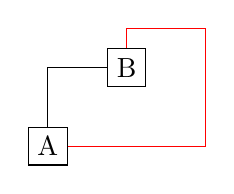
\begin{tikzpicture}
  \draw (0,0) node(a) [draw] {A}  (1,1) node(b) [draw] {B};
  \draw (a.north) |- (b.west);
  \draw[color=red] (a.east) -| (2,1.5) -| (b.north);
\end{tikzpicture}
\end{codeexample}
    %
    Instead of a coordinate you can also write \verb!cycle! to close the path:
    %

    你可以用\verb!cycle!来表示闭合路径,而不是使用坐标。



\begin{codeexample}[]
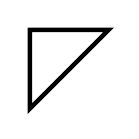
\begin{tikzpicture}[ultra thick]
  \draw (0,0) -- (1,1) -| cycle;
\end{tikzpicture}
\end{codeexample}
\end{pathoperation}

\begin{pathoperation}[noindex]{|-}{\meta{coordinate or cycle}}
    \index{--2@\protect\texttt{\protect\pgfmanualbar-} path operation}%
    \index{Path operations!--2@\protect\texttt{\protect\pgfmanualbar-}}%
    \pgfmanualpdflabel[\catcode`\|=12 ]{|-}{}%
    This operations means ``first vertical, then horizontal''.
\end{pathoperation}
}


\subsection{The Curve-To Operation\\曲线操作}

The curve-to operation allows you to extend a path using a Bézier curve.

曲线操作允许您使用贝塞尔曲线扩展路径。


\begin{pathoperation}{..}{\declare{|controls|}\meta{c}\opt{|and|\meta{d}}\declare{|..|\meta{y or cycle}}}
    This operation extends the current path from the current point, let us call
    it $x$, via a curve to a point~$y$ (if, instead of a coordinate you say
    |cycle| at the end, $y$ will be the coordinate of the last move-to
    operation). The curve is a cubic Bézier curve. For such a curve, apart
    from $y$, you also specify two control points $c$ and $d$. The idea is that
    the curve starts at $x$, ``heading'' in the direction of~$c$.
    Mathematically spoken, the tangent of the curve at $x$ goes through $c$.
    Similarly, the curve ends at $y$, ``coming from'' the other control
    point,~$d$. The larger the distance between $x$ and~$c$ and between $d$
    and~$y$, the larger the curve will be.

    此操作通过曲线从当前点$x$扩展当前路径,达到点$y$(如果在坐标处使用|cycle|代替,则$y$将成为最后一个move-to操作的坐标)。该曲线是三次贝塞尔曲线。对于这样的曲线,除了$y$,还需要指定两个控制点$c$和$d$。想法是曲线从$x$开始,指向''$c$的方向。从数学上讲,曲线在$x$处的切线通过$c$。类似地,曲线从$y$结束,来自''另一个控制点$d$。$x$和$c$之间以及$d$和$y$之间的距离越大,曲线越大。



    If the ``|and|\meta{d}'' part is not given, $d$ is assumed to be equal to
    $c$.

    如果没有给出``|and|\meta{d}''部分,则假定$d$等于$c$。

    %
\begin{codeexample}[]
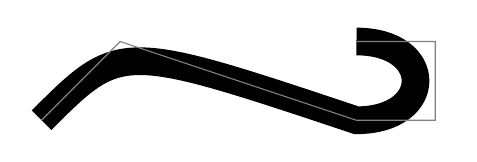
\begin{tikzpicture}
  \draw[line width=10pt] (0,0) .. controls (1,1) .. (4,0)
                               .. controls (5,0) and (5,1) .. (4,1);
  \draw[color=gray] (0,0) -- (1,1) -- (4,0) -- (5,0) -- (5,1) -- (4,1);
\end{tikzpicture}
\end{codeexample}

\begin{codeexample}[]
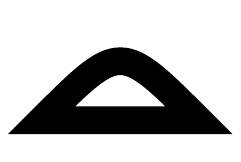
\begin{tikzpicture}
  \draw[line width=10pt] (0,0) -- (2,0) .. controls (1,1) .. cycle;
\end{tikzpicture}
\end{codeexample}

    As with the line-to operation, it makes a difference whether two curves are
    joined because they resulted from consecutive curve-to or line-to
    operations, or whether they just happen to have a common (end) point:
    %

    与线段操作类似,连接两个曲线的方式是有区别的,因为它们是由连续的曲线操作或线段操作产生的,或者它们只是碰巧有一个共同的(结束)点:

\begin{codeexample}[]
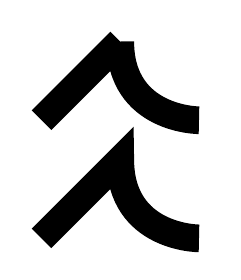
\begin{tikzpicture}[line width=10pt]
  \draw (0,0) -- (1,1) (1,1) .. controls (1,0) and (2,0) .. (2,0);
  \draw [yshift=-1.5cm]
        (0,0) -- (1,1)       .. controls (1,0) and (2,0) .. (2,0);
\end{tikzpicture}
\end{codeexample}
    %
\end{pathoperation}


\subsection{The Rectangle Operation\\矩形操作}

A rectangle can obviously be created using four straight lines and a cycle
operation. However, since rectangles are needed so often, a special syntax is
available for them.

矩形可以使用四条直线和一个cycle操作来创建。然而,由于矩形经常需要使用,因此为它们提供了特殊的语法。

\begin{pathoperation}{rectangle}{\meta{corner or cycle}}
    When this operation is used, one corner will be the current point, another
    corner is given by \meta{corner}, which becomes the new current point.
    
    当使用此操作时,一个角落将成为当前点,另一个角落由\meta{corner}给出,它成为新的当前点。

\begin{codeexample}[]
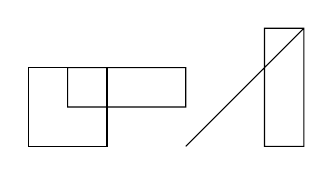
\begin{tikzpicture}
  \draw (0,0) rectangle (1,1);
  \draw (.5,1) rectangle (2,0.5) (3,0) rectangle (3.5,1.5) -- (2,0);
\end{tikzpicture}
\end{codeexample}

    Just for consistency, you can also use |cycle| instead of a coordinate, but
    it is a bit unclear what use this might have.

    为了保持一致,您也可以使用|cycle|而不是坐标,但是不太清楚这可能有什么用途。
\end{pathoperation}


\subsection{Rounding Corners\\圆角}

All of the path construction operations mentioned up to now are influenced by
the following option:

到目前为止,所有提到的路径构造操作都受以下选项的影响:

\begin{key}{/tikz/rounded corners=\meta{inset} (default 4pt)}
    When this option is in force, all corners (places where a line is continued
    either via line-to or a curve-to operation) are replaced by little arcs so
    that the corner becomes smooth.
    
当启用此选项时,所有角(通过line-to或curve-to操作继续线的位置)都将替换为小弧,使角变得平滑。
\begin{codeexample}[]
\tikz \draw [rounded corners] (0,0) -- (1,1)
           -- (2,0) .. controls (3,1) .. (4,0);
\end{codeexample}

    The \meta{inset} describes how big the corner is. Note that the
    \meta{inset} is \emph{not} scaled along if you use a scaling option like
    |scale=2|.
    %

    \meta{inset}描述了角落的大小。注意,如果使用缩放选项(如|scale=2|),则\meta{inset}不会随之缩放。


\begin{codeexample}[]
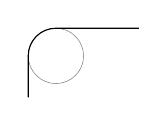
\begin{tikzpicture}
  \draw[color=gray,very thin] (10pt,15pt) circle[radius=10pt];
  \draw[rounded corners=10pt] (0,0) -- (0pt,25pt) -- (40pt,25pt);
\end{tikzpicture}
\end{codeexample}

    You can switch the rounded corners on and off ``in the middle of path'' and
    different corners in the same path can have different corner radii:
    
    在路径的中间,您可以切换圆角的开启和关闭,并且同一路径中的不同角落可以具有不同的角半径。

%
\begin{codeexample}[]
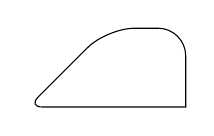
\begin{tikzpicture}
  \draw (0,0) [rounded corners=10pt] -- (1,1) -- (2,1)
                     [sharp corners] -- (2,0)
               [rounded corners=5pt] -- cycle;
\end{tikzpicture}
\end{codeexample}

    Here is a rectangle with rounded corners:

    下面是一个带有圆角的矩形:
    %
\begin{codeexample}[]
\tikz \draw[rounded corners=1ex] (0,0) rectangle (20pt,2ex);
\end{codeexample}

    You should be aware, that there are several pitfalls when using this
    option. First, the rounded corner will only be an arc (part of a circle) if
    the angle is $90^\circ$. In other cases, the rounded corner will still be
    round, but ``not as nice''.

    使用此选项时,您应该注意到存在一些陷阱。首先,只有当角度为$90^\circ$时,圆角才是一个圆弧(圆的一部分)。在其他情况下,圆角仍然是圆形的,但可能没有那么好看。

    Second, if there are very short line segments in a path, the ``rounding''
    may cause inadvertent effects. In such case it may be necessary to
    temporarily switch off the rounding using |sharp corners|.

    其次,如果路径中存在非常短的线段,则“圆角化”可能会导致意外效果。在这种情况下,可能需要使用|sharp corners|临时关闭圆角。

\end{key}

\begin{key}{/tikz/sharp corners}
    This options switches off any rounding on subsequent corners of the path.

    此选项关闭路径上后续角落的任何圆角处理。

\end{key}


\subsection{The Circle and Ellipse Operations\\圆和椭圆操作}

Circles and ellipses are common path elements for which there is a special path
operation.

圆和椭圆是常见的路径元素,可以使用特殊的路径操作来创建。

\begin{pathoperation}{circle}{\opt{|[|\meta{options}|]|}}
    This command adds a circle to the current path where the center of the
    circle is the current point by default, but you can use the |at| option to
    change this. The new current point of the path will be (typically just
    remain) the center of the circle.

    此命令向当前路径添加一个圆,其中圆心默认为当前点,但您可以使用|at|选项来更改圆心。路径的新当前点将是(通常仅保持)圆的中心。



    The radius of the circle is specified using the following options:

    圆的半径使用以下选项指定:

    %
    \begin{key}{/tikz/x radius=\meta{value}}
        Sets the horizontal radius of the circle (which, when this value is
        different form the vertical radius, is actually an ellipse). The
        \meta{value} may either be a dimension or a dimensionless number. In
        the latter case, the number is interpreted in the $xy$-coordinate
        system (if the $x$-unit is set to, say, |2cm|, then |x radius=3| will
        have the same effect as |x radius=6cm|).

        设置圆的水平半径(当此值与垂直半径不同时,实际上是一个椭圆)。 \meta{value} 可以是尺寸或无量纲数。在后一种情况下,该数字将在$xy$坐标系中解释(如果$x$单位设置为,例如,|2cm|,那么|x radius=3| 的效果与|x radius=6cm| 相同)。

    \end{key}
    %
    \begin{key}{/tikz/y radius=\meta{value}}
        Works like the |x radius|.

        与|x radius|类似。

    \end{key}
    %
    \begin{key}{/tikz/radius=\meta{value}}
        Sets the |x radius| and |y radius| simultaneously.

        同时设置|x radius|和|y radius|。

    \end{key}
    %
    \begin{key}{/tikz/at=\meta{coordinate}}
        If this option is explicitly set inside the \meta{options} (or
        indirectly via the |every circle| style), the \meta{coordinate} is used
        as the center of the circle instead of the current point. Setting |at|
        to some value in an enclosing scope has no effect.

        如果在\meta{options}内明确设置了此选项(或通过|every circle|样式间接设置),则\meta{coordinate}将用作圆的中心,而不是当前点。在封闭作用域中将|at|设置为某个值不起作用。
    \end{key}
    The \meta{options} may also contain additional options like, say, a
    |rotate| or |scale|, that will only have an effect on the circle.


    \meta{options} 还可以包含其他选项,例如|rotate|或|scale|,这些选项仅对圆有影响。
    %
\begin{codeexample}[]
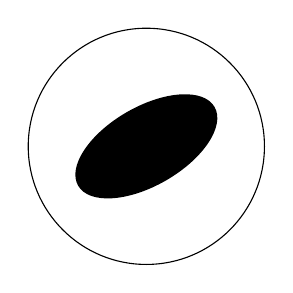
\begin{tikzpicture}
  \draw (1,0) circle [radius=1.5];
  \fill (1,0) circle [x radius=1cm, y radius=5mm, rotate=30];
\end{tikzpicture}
\end{codeexample}

    It is possible to set the |radius| also in some enclosing scope, in this
    case the options can be left out (but see the note below on what may
    follow):

    也可以在某个封闭作用域中设置|radius|,此时可以省略选项(但请参见下面关于可能跟随的说明):

    %
\begin{codeexample}[]
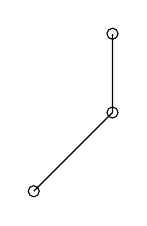
\begin{tikzpicture}[radius=2pt]
  \draw (0,0) circle -- (1,1) circle -- ++(0,1) circle;
\end{tikzpicture}
\end{codeexample}

    The following style is used with every circle:

    每个圆都使用以下样式:

    %
    \begin{stylekey}{/tikz/every circle}
        You can use this key to set up, say, a default radius for every circle.
        The key will also be used with the |ellipse| operation.

        您可以使用此键为每个圆设置默认半径。该键还将用于|ellipse|操作。

    \end{stylekey}

    In case you feel that the names |radius| and |x radius| are too long for
    your taste, you can easily created shorter aliases:
    
    如果你觉得 |radius| 和 |x radius| 这两个名字太长了,可以很容易地创建更短的别名:
    
    %
\begin{codeexample}[code only]
\tikzset{r/.style={radius=#1},rx/.style={x radius=#1},ry/.style={y radius=#1}}
\end{codeexample}
    %
    You can then say |circle [r=1cm]| or |circle [rx=1,ry=1.5]|. The reason
    \tikzname\ uses the longer names by default is that it encourages people to
    write more readable code.

    然后你可以使用 |circle [r=1cm]| 或 |circle [rx=1,ry=1.5]|。默认情况下,\tikzname\ 使用较长的名字,因为它鼓励人们编写更易读的代码。


    \emph{Note:} There also exists an older syntax for circles, where the
    radius of the circle is given in parentheses right after the |circle|
    command as in |circle (1pt)|. Although this syntax is a bit more succinct,
    it is harder to understand for readers of the code and the use of
    parentheses for something other than a coordinate is ill-chosen.

    \emph{注意:}对于圆形,还存在一种旧的语法,即在 |circle| 命令之后的括号中给出圆的半径,例如 |circle (1pt)|。虽然这种语法更加简洁,但对于代码读者来说理解起来更困难,并且使用括号表示除了坐标之外的内容是不合适的选择。


    \tikzname\ will use the following rule to determine whether the old or the
    normal syntax is used: If |circle| is directly followed by something that
    (expands to) an opening parenthesis, then the old syntax is used and inside
    these following parentheses there must be a single number or dimension
    representing a radius. In all other cases the new syntax is used.

    \tikzname\ 将使用以下规则来确定使用旧的语法还是新的语法:如果 |circle| 直接后跟某个(展开为)开括号的内容,则使用旧的语法,在这些括号内必须有一个表示半径的单个数字或尺寸。在其他所有情况下,使用新的语法。
\end{pathoperation}

\begin{pathoperation}{ellipse}{|[|\meta{options}|]|}
    This command has exactly the same effect as |circle|. The older syntax for
    this command is |ellipse (|\meta{x radius} |and| \meta{y radius}|)|. As for
    the |circle| command, this syntax is not as good as the standard syntax.
    
    
    这个命令与 |circle| 命令完全相同。该命令的旧语法是 |ellipse (|\meta{x radius} |and| \meta{y radius}|)|。与 |circle| 命令一样,这种语法不如标准语法好。
%
\begin{codeexample}[]
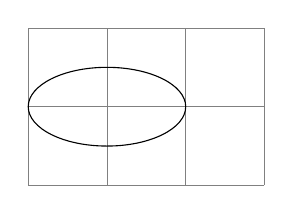
\begin{tikzpicture}
  \draw [help lines] (0,0) grid (3,2);
  \draw (1,1) ellipse [x radius=1cm,y radius=.5cm];
\end{tikzpicture}
\end{codeexample}
    %
\end{pathoperation}


\subsection{The Arc Operation\\弧操作}

The \emph{arc operation} allows you to add an arc to the current path.

\emph{弧操作}允许你在当前路径上添加一个弧。

%
\begin{pathoperation}{arc}{\oarg{options}}
    The |arc| operation adds a part of an ellipse to the current path. The
    radii of the ellipse are given by the values of |x radius| and |y radius|,
    which should be set in the \meta{options}. The arc will start at   the
    current point and will end at the end of the arc. The arc  will start and
    end at angles computed from the three keys |start angle|, |end angle|, and
    |delta angle|. Normally, the first two keys specify the start and end
    angle. However, in case one of them is empty, it is computed from the other
    key plus or minus the |delta angle|. In detail, if |end angle| is empty, it
    is set to the start angle plus the delta angle. If the start angle is
    missing, it is set to the end angle minus the delta angle. If all three
    keys are set, the delta angle is ignored.

    |arc| 操作将一个椭圆的一部分添加到当前路径中。椭圆的半径由 |x radius| 和 |y radius| 的值给出,这些值应该在 \meta{选项} 中设置。弧将从当前点开始,并在弧的结束点结束。弧的开始和结束角度由三个键 |start angle|、|end angle| 和 |delta angle| 计算得出。通常,前两个键指定起始和结束角度。然而,如果其中一个为空,它将从另一个键加上或减去 |delta angle| 来计算。具体来说,如果 |end angle| 为空,则将其设置为起始角度加上 delta angle。如果起始角度缺失,则设置为结束角度减去 delta angle。如果三个键都设置了,将忽略 delta angle。

    %
    \begin{key}{/tikz/start angle=\meta{degrees}}
        Sets the start angle.

        设置起始角度。

    \end{key}
    %
    \begin{key}{/tikz/end angle=\meta{degrees}}
        Sets the end angle.

        设置结束角度。

    \end{key}
    %
    \begin{key}{/tikz/delta angle=\meta{degrees}}
        Sets the delta angle.

        设置 delta angle。

    \end{key}

\begin{codeexample}[]
\begin{tikzpicture}[radius=1cm]
  \draw (0,0)  arc[start angle=180, end angle=90]
     -- (2,.5) arc[start angle=90,  delta angle=-90];
  \draw (4,0) -- +(30:1cm)
              arc [start angle=30,  delta angle=30] -- cycle;
  \draw (8,0) arc [start angle=0,   end angle=270,
                   x radius=1cm, y radius=5mm] -- cycle;
\end{tikzpicture}
\end{codeexample}

\begin{codeexample}[]
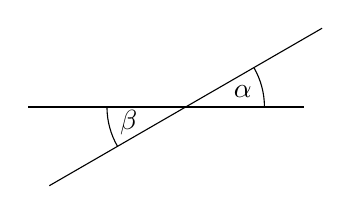
\begin{tikzpicture}[radius=1cm,delta angle=30]
  \draw (-1,0) -- +(3.5,0);
  \draw (1,0) ++(210:2cm) -- +(30:4cm);
  \draw (1,0) +(0:1cm) arc [start angle=0];
  \draw (1,0) +(180:1cm) arc [start angle=180];
  \path (1,0) ++(15:.75cm) node{$\alpha$};
  \path (1,0) ++(15:-.75cm) node{$\beta$};
\end{tikzpicture}
\end{codeexample}

    There also exists a shorter syntax for the arc operation, namely |arc|
    begin directly followed by
    |(|\meta{start angle}|:|\meta{end angle}|:|\meta{radius}). However, this
    syntax is harder to read, so the normal syntax should be preferred in
    general.

    弧操作还存在一种更短的语法,即 |arc| 直接后跟 |(|\meta{起始角度}|:|\meta{结束角度}|:|\meta{半径})。然而,这种语法更难阅读,因此通常应优先使用标准语法。

\end{pathoperation}


\subsection{The Grid Operation\\网格操作}

You can add a grid to the current path using the |grid| path operation.

你可以使用 |grid| 路径操作在当前路径中添加一个网格。


\begin{pathoperation}{grid}{\opt{\oarg{options}}\meta{corner or cycle}}
    This operations adds a grid filling a rectangle whose two corners are given
    by \meta{corner} and by the previous coordinate. (Instead of a coordinate
    you can also say |cycle| to use the position of the last move-to as the
    corner coordinate, but it not very natural to do so.) Thus, the
    typical way in which a grid is drawn is |\draw (1,1) grid (3,3);|, which
    yields a grid filling the rectangle whose corners are at $(1,1)$ and
    $(3,3)$. All coordinate transformations apply to the grid.
    %

    这个操作在一个由 \meta{角} 和前一个坐标给出的矩形中添加一个网格。(你也可以使用 |cycle| 来表示最后一个移动到的位置作为角坐标,但这并不是很自然。)因此,绘制网格的典型方式是 |\draw (1,1) grid (3,3);|,它生成填充角坐标为$(1,1)$和$(3,3)$的矩形网格。所有坐标变换都适用于网格。

\begin{codeexample}[]
\tikz[rotate=30] \draw[step=1mm] (0,0) grid (2,2);
\end{codeexample}

    The \meta{options}, which are local to the |grid| operation, can be used to
    influence the appearance of the grid. The stepping of the grid is governed
    by the following options:

    \meta{选项}是局部于 |grid| 操作的,可以用来影响网格的外观。网格的步进由以下选项控制:

    %
    \begin{key}{/tikz/step=\meta{number or dimension or coordinate} (initially 1cm)}
        Sets the stepping in both the $x$ and $y$-direction. If a dimension is
        provided, this is used directly. If a number is provided, this number
        is interpreted in the $xy$-coordinate system. For example, if you
        provide the number |2|, then the $x$-step is twice the $x$-vector and
        the $y$-step is twice the $y$-vector set by the |x=| and |y=| options.
        Finally, if you provide a coordinate, then the $x$-part of this
        coordinate will be used as the $x$-step and the $y$-part will be used
        as the $y$-coordinate.

        设置$x$和$y$方向的步进。如果提供了尺寸,则直接使用该尺寸。如果提供了数字,则该数字将在$xy$坐标系中解释。例如,如果提供数字|2|,则$x$步进是$x$向量的两倍,$y$步进是$y$向量的两倍,这些向量由|x=|和|y=|选项设置。最后,如果提供了一个坐标,则该坐标的$x$部分将用作$x$步进,$y$部分将用作$y$坐标。
        %
\begin{codeexample}[]
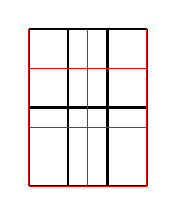
\begin{tikzpicture}[x=.5cm]
  \draw[thick] (0,0) grid [step=1]     (3,2);
  \draw[red]   (0,0) grid [step=.75cm] (3,2);
\end{tikzpicture}
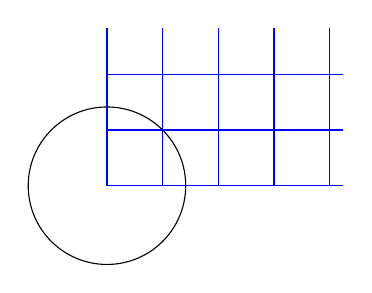
\begin{tikzpicture}
  \draw        (0,0) circle [radius=1];
  \draw[blue]  (0,0) grid [step=(45:1)] (3,2);
\end{tikzpicture}
\end{codeexample}

        A complication arises when the $x$- and/or $y$-vector do not point
        along the axes. Because of this, the actual rule for computing the
        $x$-step and the $y$-step is the following: As the $x$- and $y$-steps
        we use the $x$- and $y$-components or the following two vectors: The
        first vector is either $(\meta{x-grid-step-number},0)$ or
        $(\meta{x-grid-step-dimension},0\mathrm{pt})$, the second vector is
        $(0,\meta{y-grid-step-number})$ or
        $(0\mathrm{pt},\meta{y-grid-step-dimension})$.

        当$x$和/或$y$向量不指向坐标轴时,会出现一个复杂性。因此,计算$x$步进和$y$步进的实际规则如下:我们将$x$步进和$y$步进作为以下两个向量的$x$和$y$分量使用:第一个向量可以是$(\meta{x-grid-step-number},0)$或$(\meta{x-grid-step-dimension},0\mathrm{pt})$,第二个向量是$(0,\meta{y-grid-step-number})$或$(0\mathrm{pt},\meta{y-grid-step-dimension})$。

        If the $x$-step or $y$-step is $0$ or negative the corresponding lines
        are not drawn.

        如果$x$步进或$y$步进为$0$或负数,则不绘制相应的线条。
    \end{key}

    \begin{key}{/tikz/xstep=\meta{dimension or number} (initially 1cm)}
        Sets the stepping in the $x$-direction.

        设置$x$方向的步进。
        %
\begin{codeexample}[]
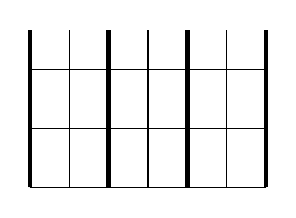
\begin{tikzpicture}
  \draw (0,0) grid [xstep=.5,ystep=.75] (3,2);
  \draw[ultra thick] (0,0) grid [ystep=0] (3,2);
\end{tikzpicture}
\end{codeexample}
    \end{key}

    \begin{key}{/tikz/ystep=\meta{dimension or number} (initially 1cm)}
        Sets the stepping in the $y$-direction.

        设置$y$方向的步进。
    \end{key}

    It is important to note that the grid is always ``phased'' such that it
    contains the point $(0,0)$ if that point happens to be inside the
    rectangle. Thus, the grid does \emph{not} always have an intersection at
    the corner points; this occurs only if the corner points are multiples of
    the stepping. Note that due to rounding errors, the ``last'' lines of a
    grid may be omitted. In this case, you have to add an epsilon to the corner
    points.

    重要的是要注意,网格总是“分阶段”的,以便包含点$(0,0)$,如果该点恰好位于矩形内部。因此,网格不一定在角点处交叉;只有当角点是步进的倍数时才会发生交叉。注意,由于舍入误差,网格的“最后”线可能会被省略。在这种情况下,你需要在角点上添加一个 epsilon。

    The following style is useful for drawing grids:

    以下样式对绘制网格很有用:

    %
    \begin{stylekey}{/tikz/help lines (initially {line width=0.2pt,gray})}
        This style makes lines ``subdued'' by using thin gray lines for them.
        However, this style is not installed automatically and you have to say
        for example:

        该样式通过使用细灰色线条使线条“平淡”。然而,该样式不会自动安装,你需要手动设置,例如:
        %
\begin{codeexample}[]
\tikz \draw[help lines] (0,0) grid (3,3);
\end{codeexample}
    \end{stylekey}
\end{pathoperation}


\subsection{The Parabola Operation\\抛物线操作}

The |parabola| path operation continues the current path with a parabola. A
parabola is a (shifted and scaled) curve defined by the equation $f(x) = x^2$
and looks like this: \tikz \draw (-1ex,1.5ex) parabola[parabola height=-1.5ex]
+(2ex,0ex);.

|parabola|路径操作可以延续当前路径并绘制一条抛物线。抛物线是由方程 $f(x) = x^2$ 定义的(平移和缩放后的)曲线,如下所示:\tikz \draw (-1ex,1.5ex) parabola[parabola height=-1.5ex] +(2ex,0ex);。

\begin{pathoperation}{parabola}{\opt{\oarg{options}|bend|\meta{bend
        coordinate}}\meta{coordinate or cycle}}
    This operation adds a parabola through the current point and the given
    \meta{coordinate} or, if |cycle| is used instead of coordinate at the end,
    the \meta{coordinate} is set to the position of the last move-to and the
    path gets closed after the parabola. If the |bend| is given, it specifies
    where the bend should go; the \meta{options} can also be used to specify
    where the bend is. By default, the bend is at the old current point.
    %

    此操作通过当前点和给定的\meta{坐标}(如果在末尾使用 |cycle| 代替坐标,则将\meta{坐标}设置为最后一个移动到的位置,并在抛物线后关闭路径)添加一条抛物线。如果给出了 |bend|,它指定了弯曲的位置;\meta{选项}也可用于指定弯曲的位置。默认情况下,弯曲点位于旧的当前点。
\begin{codeexample}[]
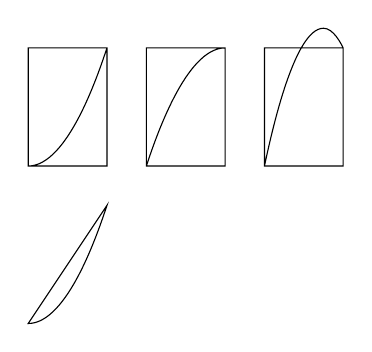
\begin{tikzpicture}
  \draw                (0,0) rectangle                (1,1.5)
                       (0,0) parabola                 (1,1.5);
  \draw[xshift=1.5cm]  (0,0) rectangle                (1,1.5)
                       (0,0) parabola[bend at end]    (1,1.5);
  \draw[xshift=3cm]    (0,0) rectangle                (1,1.5)
                       (0,0) parabola bend (.75,1.75) (1,1.5);

  \draw[yshift=-2cm]   (1,1.5) --
                       (0,0) parabola                 cycle;
\end{tikzpicture}
\end{codeexample}

    The following options influence parabolas:

    以下选项影响抛物线:

    %
    \begin{key}{/tikz/bend=\meta{coordinate}}
        Has the same effect as saying |bend|\meta{coordinate} outside the
        \meta{options}. The option specifies that the bend of the parabola
        should be at the given \meta{coordinate}. You have to take care
        yourself that the bend position is a ``valid'' position; which means
        that if there is no parabola of the form $f(x) = a x^2 + b x + c$ that
        goes through the old current point, the given bend, and the new current
        point, the result will not be a parabola.

        具有与在\meta{选项}之外使用 |bend|\meta{坐标} 相同的效果。该选项指定抛物线的弯曲应位于给定的\meta{坐标}处。您必须自行确保弯曲位置是一个“有效”的位置;这意味着如果不存在形式为 $f(x) = a x^2 + b x + c$ 的抛物线通过旧的当前点、给定的弯曲点和新的当前点,则结果将不是抛物线。


        There is one special property of the \meta{coordinate}: When a relative
        coordinate is given like |+(0,0)|, the position relative to this
        coordinate is ``flexible''. More precisely, this position lies
        somewhere on a line from the old current point to the new current
        point. The exact position depends on the next option.

        \meta{坐标}有一个特殊属性:当给出一个相对坐标,如 |+(0,0)|,该位置相对于此坐标是“灵活的”。更准确地说,此位置位于从旧的当前点到新的当前点的直线上的某个位置。确切的位置取决于下一个选项。

    \end{key}

    \begin{key}{/tikz/bend pos=\meta{fraction}}
        Specifies where the ``previous'' point is relative to which the bend is
        calculated. The previous point will be at the \meta{fraction}th part of
        the line from the old current point to the new current point.

        指定“前一个”点相对于其中计算弯曲的点的位置。前一个点将位于从旧的当前点到新的当前点的直线的第 \meta{分数} 部分处。


        The idea is the following: If you say |bend pos=0| and |bend +(0,0)|,
        the bend will be at the old current point. If you say |bend pos=1| and
        |bend +(0,0)|, the bend will be at the new current point. If you say
        |bend pos=0.5| and |bend +(0,2cm)| the bend will be 2cm above the
        middle of the line between the start and end point. This is most useful
        in situations such as the following:

        思路如下:如果您设置了 |bend pos=0| 和 |bend +(0,0)|,则弯曲将位于旧的当前点。如果您设置了 |bend pos=1| 和 |bend +(0,0)|,则弯曲将位于新的当前点。如果您设置了 |bend pos=0.5| 和 |bend +(0,2cm)|,则弯曲将位于起始点和结束点之间的中线上方 2cm 处。这在以下情况下非常有用:

        %
\begin{codeexample}[]
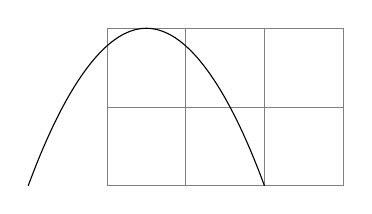
\begin{tikzpicture}
  \draw[help lines] (0,0) grid (3,2);
  \draw (-1,0) parabola[bend pos=0.5] bend +(0,2) +(3,0);
\end{tikzpicture}
\end{codeexample}

        In the above example, the |bend +(0,2)| essentially means ``a parabola
        that is 2cm high'' and |+(3,0)| means ``and 3cm wide''. Since this
        situation arises often, there is a special shortcut option:

        在上面的示例中,|bend +(0,2)| 的效果实际上是“一个高度为 2cm 的抛物线”,而 |+(3,0)| 的效果是“宽度为 3cm”。由于这种情况经常出现,有一个特殊的快捷选项:

        %
        \begin{key}{/tikz/parabola height=\meta{dimension}}
            This option has the same effect as          |[bend pos=0.5,bend={+(0pt,|\meta{dimension}|)}]|.

            此选项的效果与 |[bend pos=0.5,bend={+(0pt,|\meta{尺寸}|)}]| 相同。

            %
\begin{codeexample}[]
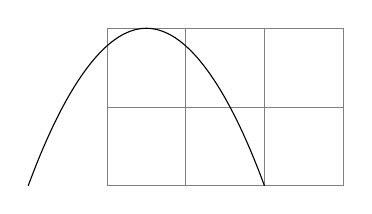
\begin{tikzpicture}
  \draw[help lines] (0,0) grid (3,2);
  \draw (-1,0) parabola[parabola height=2cm] +(3,0);
\end{tikzpicture}
\end{codeexample}
        \end{key}
    \end{key}

    The following styles are useful shortcuts:

    以下样式是有用的快捷方式:

    %
    \begin{stylekey}{/tikz/bend at start}
        This places the bend at the start of a parabola. It is a shortcut for
        the following options: |bend pos=0,bend={+(0,0)}|.

        将弯曲放置在抛物线的起点。这是以下选项的快捷方式:|bend pos=0,bend={+(0,0)}|。
    \end{stylekey}

    \begin{stylekey}{/tikz/bend at end}
        This places the bend at the end of a parabola.

        将弯曲放置在抛物线的终点。
    \end{stylekey}
\end{pathoperation}


\subsection{The Sine and Cosine Operation\\正弦和余弦操作}

The |sin| and |cos| operations are similar to the |parabola| operation. They,
too, can be used to draw (parts of) a sine or cosine curve.

|sin|和|cos|操作类似于|parabola|操作。它们也可以用于绘制正弦曲线或余弦曲线的(部分)路径。


\begin{pathoperation}{sin}{\meta{coordinate or cycle}}
    The effect of |sin| is to draw a scaled and shifted version of a sine curve
    in the interval $[0,\pi/2]$. The scaling and shifting is done in such a way
    that the start of the sine curve in the interval is at the old current
    point and that the end of the curve in the interval is at
    \meta{coordinate}. Here is an example that should clarify this:

    |sin| 的作用是在区间 $[0,\pi/2]$ 上绘制一个经过缩放和平移的正弦曲线。缩放和平移是这样进行的:在区间中,曲线的起点位于旧的当前点,并且曲线的终点位于\meta{坐标}处。以下是一个可以说明的示例:
    %
\begin{codeexample}[]
\tikz \draw (0,0) rectangle (1,1)     (0,0) sin (1,1)
            (2,0) rectangle +(1.57,1) (2,0) sin +(1.57,1);
\end{codeexample}
    %
\end{pathoperation}

\begin{pathoperation}{cos}{\meta{coordinate or cycle}}
    This operation works similarly, only a cosine in the interval $[0,\pi/2]$
    is drawn. By correctly alternating |sin| and |cos| operations, you can
    create a complete sine or cosine curve:

    此操作类似,只是绘制的是 $[0,\pi/2]$ 区间内的余弦曲线。通过正确交替使用 |sin| 和 |cos| 操作,您可以创建完整的正弦或余弦曲线:

    %
\begin{codeexample}[]
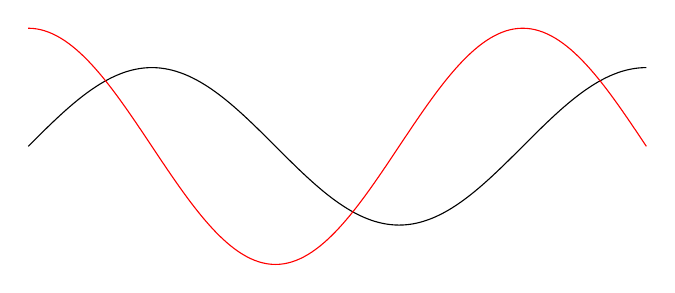
\begin{tikzpicture}[xscale=1.57]
  \draw (0,0) sin (1,1) cos (2,0) sin (3,-1) cos (4,0) sin (5,1);
  \draw[color=red] (0,1.5) cos (1,0) sin (2,-1.5) cos (3,0) sin (4,1.5) cos (5,0);
\end{tikzpicture}
\end{codeexample}
    %
\end{pathoperation}

Note that there is no way to (conveniently) draw an interval on a sine or
cosine curve whose end points are not multiples of $\pi/2$.

请注意,没有一种(便捷的)方法可以绘制正弦或余弦曲线上端点不是 $\pi/2$ 的区间。


\subsection{The SVG Operation\\SVG操作}

The |svg| operation can be used to extend the current path by a path given in
the \textsc{svg} path data syntax. This syntax is described in detail in
Section~8.3 of the \textsc{svg 1.1} specification, please consult this
specification for details.

|svg|操作可用于使用\textsc{svg}路径数据语法在当前路径上扩展路径。该语法在\textsc{svg 1.1}规范的第8.3节中详细描述,请参考该规范获取详细信息。


\begin{pathoperation}{svg}{\opt{\oarg{options}}\marg{path data}}
    This operation adds the path specified in the \meta{path data} in
    \textsc{svg 1.1 path data} syntax to the current path. Unlike the
    \textsc{svg}-specification, it \emph{is} permissible that the path data
    does not start with a move-to command (|m| or |M|), in which case the last
    point of the current path is used as start point. The optional
    \meta{options} apply locally to this path operation, typically you will use
    them to set up, say, some transformations.

    此操作将以\textsc{svg 1.1路径数据}语法中指定的路径添加到当前路径中。与\textsc{svg}规范不同,路径数据可以不以移动到命令(|m|或|M|)开头,在这种情况下,当前路径的最后一个点将作为起始点。可选的\meta{选项}仅适用于此路径操作的局部,通常您将使用它们来设置某些变换。

    %
\begin{codeexample}[preamble={\usetikzlibrary{svg.path}}]
\begin{tikzpicture}
  \filldraw [fill=red!20] (0,1) svg[scale=2] {h 10 v 10 h -10}
    node [above left] {upper left} -- cycle;

  \draw svg {M 0 0 L 20 20 h 10 a 10 10 0 0 0 -20 0};
\end{tikzpicture}
\end{codeexample}

    An \textsc{svg} coordinate like |10 20| is always interpreted as
    |(10pt,20pt)|, so the basic unit is always points (|pt|). The
    $xy$-coordinate system is not used. However, you can use scaling to
    (locally) change the basic unit. For instance, |svg[scale=1cm]| (yes, this
    works, although some rather evil magic is involved) will cause 1cm to be
    the basic unit.

    \textsc{svg}坐标,如|10 20|,始终被解释为|(10pt,20pt)|,因此基本单位始终为点(|pt|)。不使用$xy$坐标系。但是,您可以使用缩放来(局部地)更改基本单位。例如,|svg[scale=1cm]|(是的,这有效,尽管涉及某种黑魔法)将导致1cm成为基本单位。


    Instead of curly braces, you can also use quotation marks to indicate the
    start and end of the \textsc{svg} path.

    您还可以使用引号而不是花括号来指示\textsc{svg}路径的起始和结束。


    \emph{Warning:} The arc operations (|a| and |A|) are  numerically instable.
    This means that they will be quite imprecise, except when the angle is a
    multiple of $90^\circ$ (as is, fortunately, most often the case).

    \emph{警告:}弧线操作(|a|和|A|)在数值上是不稳定的。这意味着它们会相当不精确,除非角度是$90^\circ$的倍数(幸运的是,这种情况最常见)。

\end{pathoperation}


\subsection{The Plot Operation\\绘图操作}

The |plot| operation can be used to append a line or curve to the path that
goes through a large number of coordinates. These coordinates are either given
in a simple list of coordinates, read from some file, or they are computed on
the fly.

|plot| 操作可用于将线条或曲线添加到经过大量坐标的路径上。这些坐标可以通过简单的坐标列表给出,从某个文件中读取,或者在运行时计算得出。



Since the syntax and the behavior of this command are a bit complex, they are
described in the separated Section~\ref{section-tikz-plots}.

由于该命令的语法和行为有些复杂,因此在单独的第~\ref{section-tikz-plots} 节中对其进行了描述。


\subsection{The To Path Operation\\路径操作}

The |to| operation is used to add a user-defined path from the previous
coordinate to the following coordinate. When you write |(a) to (b)|, a straight
line is added from |a| to |b|, exactly as if you had written |(a) -- (b)|.
However, if you write |(a) to [out=135,in=45] (b)| a curve is added to the
path, which leaves at an angle of 135$^\circ$ at |a| and arrives at an angle of
45$^\circ$ at |b|. This is because the options |in| and |out| trigger a special
path to be used instead of the straight line.

|to| 操作用于从前一个坐标到后一个坐标添加用户定义的路径。当你写 |(a) to (b)| 时,会添加一条从 |a| 到 |b| 的直线,就像你写了 |(a) -- (b)| 一样。然而,如果你写了 |(a) to [out=135,in=45] (b)|,则会添加一条曲线路径,该路径从 |a| 处以 135$^\circ$ 的角度离开,并以 45$^\circ$ 的角度到达 |b|。这是因为选项 |in| 和 |out| 触发了特殊的路径,而不是直线。



\begin{pathoperation}{to}{\opt{|[|\meta{options}|]|}
        \opt{\meta{nodes}} \meta{coordinate or cycle}}
    This path operation inserts the path currently set via the |to path| option
    at the current position. The \meta{options} can be used to modify (perhaps
    implicitly) the |to path| and to set up how the path will be rendered.

    此路径操作在当前位置插入当前通过 |to path| 选项设置的路径。\meta{选项}可用于修改(可能是隐式地)|to path| 并设置路径的渲染方式。


    Before the |to path| is inserted, a number of macros are set up that can
    ``help'' the |to path|. These are |\tikztostart|, |\tikztotarget|, and
    |\tikztonodes|; they are explained in the following.

    在插入 |to path| 之前,会设置一些宏,这些宏可以“帮助”|to path|。它们是 |\tikztostart|、|\tikztotarget| 和 |\tikztonodes|;以下将对它们进行解释。


    \medskip
    \textbf{Start and Target Coordinates.}\ \
    The |to| operation is always followed by a \meta{coordinate}, called the
    target coordinate, or the text |cycle|, in which case the last move-to is
    used as a coordinate and the path gets closed. The macro |\tikztotarget| is
    set to this coordinate (without its parentheses). There is also a
    \emph{start coordinate}, which is the coordinate preceding the |to|
    operation. This coordinate can be accessed via the macro |\tikztostart|. In
    the following example, for the first |to|, the macro |\tikztostart| is
    |0pt,0pt| and the |\tikztotarget| is |0,2|. For the second |to|, the macro
    |\tikztostart| is |10pt,10pt| and |\tikztotarget| is |a|. For the third,
    they are set to |a| and |current subpath start|.

    \textbf{起始坐标和目标坐标。}\ \
|to| 操作后始终跟着一个称为目标坐标的 \meta{坐标},或者文本 |cycle|,在这种情况下,最后的移动到将用作坐标并关闭路径。宏 |\tikztotarget| 被设置为此坐标(不包括其括号)。还有一个\emph{起始坐标},即 |to| 操作之前的坐标。可以通过宏 |\tikztostart| 访问此坐标。在下面的示例中,第一个 |to| 的宏 |\tikztostart| 是 |0pt,0pt|,而 |\tikztotarget| 是 |0,2|。第二个 |to| 的宏 |\tikztostart| 是 |10pt,10pt|,而 |\tikztotarget| 是 |a|。对于第三个 |to|,它们分别设置为 |a| 和 |current subpath start|。

    %
\begin{codeexample}[]
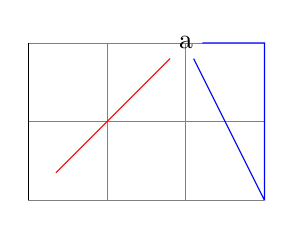
\begin{tikzpicture}
  \draw[help lines] (0,0) grid (3,2);
  \node       (a)         at (2,2) {a};

  \draw       (0,0)       to (0,2);
  \draw[red]  (10pt,10pt) to (a);
  \draw[blue] (3,0) -- (3,2) -- (a) to cycle;
\end{tikzpicture}
\end{codeexample}

    \medskip
    \textbf{Nodes on to--paths.}\ \
    It is possible to add nodes to the paths constructed by a |to| operation.
    To do so, you specify the nodes between the |to| keyword and the coordinate
    (if there are options to the |to| operation, these come first). The effect
    of |(a) to node {x} (b)| (typically) is the same as if you had written
    |(a) -- node {x} (b)|, namely that the node is placed on the |to|. This can
    be used to add labels to |to|s:

    \textbf{to--路径上的节点。}\ \
可以将节点添加到 |to| 操作构建的路径中。为此,你需要在 |to| 关键字和坐标之间指定节点(如果有 |to| 操作的选项,则首先使用这些选项)。|(a) to node {x} (b)|(通常)的效果与你写了 |(a) -- node {x} (b)| 相同,即该节点被放置在 |to| 上。这可用于添加标签到 |to| 上:
    %
\begin{codeexample}[]
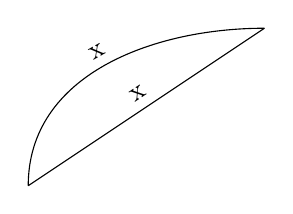
\begin{tikzpicture}
  \draw (0,0) to node [sloped,above] {x} (3,2);

  \draw (0,0) to[out=90,in=180] node [sloped,above] {x} (3,2);
\end{tikzpicture}
\end{codeexample}

    Instead of writing the node between the |to| keyword and the target
    coordinate, you may also use the following keys to create such nodes:

    你还可以使用以下键来在 |to| 关键字和目标坐标之间创建这些节点:

    %
    \begin{key}{/tikz/edge node=\meta{node specification}}
        This key can be used inside the \meta{options} of a |to| path command.
        It will add the \meta{node specification} to the list of nodes to be
        placed on the connecting line, just as if you had written the
        \meta{node specification} directly after the |to| keyword:

        此键可在 |to| 路径命令的 \meta{选项} 中使用。它将 \meta{节点规范} 添加到要放置在连接线上的节点列表中,就好像你直接在 |to| 关键字之后写了 \meta{节点规范} 一样:

        %
\begin{codeexample}[]
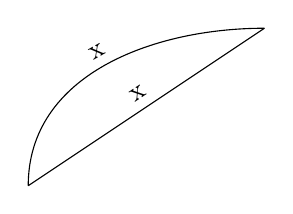
\begin{tikzpicture}
  \draw (0,0) to [edge node={node [sloped,above] {x}}] (3,2);

  \draw (0,0) to [out=90,in=180,
                  edge node={node [sloped,above] {x}}] (3,2);
\end{tikzpicture}
\end{codeexample}
        %
        This key is mostly useful to create labels automatically using other
        keys.
        
        这个选项通常用于使用其他选项自动创建标签。


    \end{key}
    %
    \begin{key}{/tikz/edge label=\meta{text}}
        A shorthand for |edge node={node[auto]{|\meta{text}|}}|.

        是 |edge node={node[auto]{|\meta{text}|}}| 的简写形式。

        %
\begin{codeexample}[]
\tikz \draw (0,0) to [edge label=x] (3,2);
\end{codeexample}
    \end{key}
    %
    \begin{key}{/tikz/edge label'=\meta{text}}
        A shorthand for |edge node={node[auto,swap]{|\meta{text}|}}|.

        是 |edge node={node[auto,swap]{|\meta{text}|}}| 的简写形式。

        %
\begin{codeexample}[]
\tikz \draw (0,0) to [edge label=x, edge label'=y] (3,2);
\end{codeexample}
    \end{key}

    When the |quotes| library is loaded, additional ways of specifying nodes on
    to--paths become available, see Section~\ref{section-edge-quotes}.

    当加载 |quotes| 库时,可以使用其他方式来指定 to--paths 上的节点,参见第~\ref{section-edge-quotes}~节。

    \medskip
    \textbf{Styles for to-paths.}\ \
    In addition to the \meta{options} given after the |to| operation, the
    following style is also set at the beginning of the to path:

    \textbf{to-paths 的样式。}\ \
除了在 |to| 操作后给出的 \meta{options} 外,还有以下样式在 to path 的开始处设置:
    %
    \begin{stylekey}{/tikz/every to (initially \normalfont empty)}
        This style is installed at the beginning of every to.

        这个样式被应用于每个 to 的开头。
        %
\begin{codeexample}[]
\tikz[every to/.style={bend left}]
  \draw (0,0) to (3,2);
\end{codeexample}
        %
        Note that, as explained below, every to path is implicitly surrounded
        by curly braces. This means that options like |draw| given in an
        |every to| do not actually influence the path. You can fix this by
        using the |append after command| option:

        注意,如下所述,每个 to path 隐式地由花括号包围。这意味着在 |every to| 中给出的诸如 |draw| 的选项实际上并不影响路径。可以通过使用 |append after command| 选项来解决这个问题:

        %
\begin{codeexample}[]
\tikz[every to/.style={append after command={[draw,dashed]}}]
  \draw (0,0) to (3,2);
\end{codeexample}
    \end{stylekey}

    \medskip
    \textbf{Options.}\ \
    The \meta{options} given with the |to| allow you to influence the
    appearance of the |to path|. Mostly, these options are used to change the
    |to path|. This can be used to change the path from a straight line to,
    say, a curve.

    \textbf{选项。}\ \
与 |to| 一起给出的 \meta{options} 允许你影响 |to path| 的外观。主要用于改变 |to path|,可以将直线路径更改为曲线路径等。

    The path used is set using the following option:

    使用以下选项设置路径:

    %
    \begin{key}{/tikz/to path=\meta{path}}
        Whenever a |to| operation is used, the \meta{path} is inserted. More
        precisely, the following path is added:

        每当使用 |to| 操作时,都会插入 \meta{path}。更准确地说,添加以下路径:

        %
        \begin{quote}
            |{[every to,|\meta{options}|] |\meta{path} |}|
        \end{quote}

        The \meta{options} are the options given to the |to| operation, the
        \meta{path} is the path set by this option |to path|.

        \meta{options} 是给 |to| 操作的选项,\meta{path} 是由选项 |to path| 设置的路径。


        Inside the \meta{path}, different macros are used to reference the
        from- and to-coordinates. In detail, these are:

        在 \meta{path} 中,使用不同的宏来引用起点和终点坐标。具体来说,它们是:

        %
        \begin{itemize}
            \item \declareandlabel{\tikztostart} will expand to the
                from-coordinate (without the parentheses).

                \declareandlabel{\tikztostart} 会展开为起点坐标(不包括括号)。
            \item \declareandlabel{\tikztotarget} will expand to the
                to-coordinate.

                \declareandlabel{\tikztotarget} 会展开为终点坐标。
            \item \declareandlabel{\tikztonodes} will expand to the nodes
                between the |to| operation and the coordinate. Furthermore,
                these nodes will have the |pos| option set implicitly.

                \declareandlabel{\tikztonodes} 会展开为 |to| 操作和坐标之间的节点。此外,这些节点将隐式设置 |pos| 选项。
        \end{itemize}

        Let us have a look at a simple example. The standard straight line for
        a |to| is achieved by the following \meta{path}:

        现在让我们来看一个简单的例子。|to| 的标准直线由以下 \meta{path} 实现:

        %
        \begin{quote}
            |-- (\tikztotarget) \tikztonodes|
        \end{quote}

        Indeed, this is the default setting for the path. When we write
        |(a) to (b)|, the \meta{path} will expand to |(a) -- (b)|, when we
        write

        的确,这是路径的默认设置。当我们写
        |(a) to (b)| 时,\meta{path} 展开为 |(a) -- (b)|,当我们写
    
        %
        \begin{quote}
            |(a) to[red] node {x} (b)|
        \end{quote}
        %
        the \meta{path} will expand to

        \meta{path} 展开为

        %
        \begin{quote}
            |(a) -- (b) node[red] {x}|
        \end{quote}

        It is not possible to specify the path

        无法指定路径

        %
        \begin{quote}
            |-- \tikztonodes (\tikztotarget)|
        \end{quote}
        %
        since \tikzname\ does not allow one to have a macro after |--| that
        expands to a node.

        因为 \tikzname\ 不允许在 |--| 后使用展开为节点的宏。


        Now let us have a look at how we can modify the \meta{path} sensibly.
        The simplest way is to use a curve.
        %

        现在让我们看看如何合理修改 \meta{path}。最简单的方法是使用曲线。

\begin{codeexample}[]
\begin{tikzpicture}[to path={
    .. controls +(1,0) and +(1,0) .. (\tikztotarget) \tikztonodes}]

  \node (a) at (0,0) {a};
  \node (b) at (2,1) {b};
  \node (c) at (1,2) {c};

  \draw (a) to node {x} (b)
        (a) to          (c);
\end{tikzpicture}
\end{codeexample}

        Here is another example:

        这里是另一个例子:

        %
\begin{codeexample}[]
\tikzset{
  my loop/.style={to path={
    .. controls +(80:1) and +(100:1) .. (\tikztotarget) \tikztonodes}},
  my state/.style={circle,draw}}

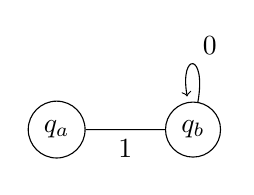
\begin{tikzpicture}[shorten >=2pt]
  \node [my state] (a) at (210:1) {$q_a$};
  \node [my state] (b) at (330:1) {$q_b$};

  \draw[->] (a) to           node[below]       {1} (b)
                to [my loop] node[above right] {0} (b);
\end{tikzpicture}
\end{codeexample}

        \begin{key}{/tikz/execute at begin to=\meta{code}}
            The \meta{code} is executed prior to the |to|. This can be used to
            draw one or more additional paths or to do additional computations.

            在 |to| 之前执行 \meta{code}。这可以用来绘制一个或多个附加路径,或进行其他计算。

        \end{key}

        \begin{key}{/tikz/execute at end to=\meta{code}}
            Works like the previous option, only this code is executed after
            the to path has been added.
            % FIXME : provide examples...

            类似于前一个选项,只是这个代码在添加 to path 后执行。% FIXME : 提供示例...
        \end{key}

        \begin{stylekey}{/tikz/every to (initially \normalfont empty)}
            This style is installed at the beginning of every to.

            这个样式被应用于每个 to 的开头。

        \end{stylekey}
    \end{key}
\end{pathoperation}

There are a number of predefined |to path|s, see Section~\ref{library-to-paths}
for a reference.

有一些预定义的 |to path|s,参见第~\ref{library-to-paths}~节进行了参考。



\subsection{The Foreach Operation\\Foreach操作}

\begin{pathoperation}{foreach}{\meta{variables}\opt{\oarg{options}} |in|
        \marg{path commands}}
    The |foreach| operation can be used to repeatedly insert the \meta{path
    commands} into the current path. Naturally, the \meta{path commands} should
    internally reference some of the \meta{variables} so that you do not insert
    exactly the same path repeatedly, but rather variations. For historical
    reasons, you can also write |\foreach| instead of |foreach|.
    
    |foreach|操作可用于将\meta{path commands}重复插入当前路径中。自然地,\meta{path commands}应在内部引用一些\meta{variables},以便您不是重复插入完全相同的路径,而是变体。出于历史原因,您也可以写成|\foreach|而不是|foreach|。

\begin{codeexample}[]
\tikz \draw (0,0) foreach \x in {1,...,3} { -- (\x,1) -- (\x,0) };
\end{codeexample}
    %
    See Section~\ref{section-foreach} for more details on the for-each-command.

    更多关于for-each命令的详细信息,请参见第~\ref{section-foreach}节。

\end{pathoperation}


\subsection{The Let Operation\\Let操作}

The \emph{let operation} is the first of a number of path operations that do
not actually extend that path, but have different, mostly local, effects.
It requires the |calc| library, see Section~\ref{tikz-lib-calc}.

\emph{let操作}是一系列不实际扩展路径但具有不同(主要是局部)效果的路径操作之一。它需要|calc|库,请参见第~\ref{tikz-lib-calc}节。

\begin{pathoperation}{let}{\meta{assignment}
        \opt{|,|\meta{assignment}}%
        \opt{|,|\meta{assignment}\dots}\declare{| in |}}
    When this path operation is encountered, the \meta{assignment}s are
    evaluated, one by one. This will store coordinate and number in
    special \emph{registers} (which are local to \tikzname, they have
    nothing to do with \TeX\ registers). Subsequently, one can access the
    contents of these registers using the macros |\p|, |\x|, |\y|, and
    |\n|.

    当遇到此路径操作时,将逐个计算\meta{assignment}。这将把坐标和数字存储在特殊的\emph{寄存器}中(这些寄存器是局部于\tikzname 的,与\TeX 寄存器无关)。随后,可以使用宏|\p|、|\x|、|\y|和|\n|访问这些寄存器的内容。


    The first kind of permissible \meta{assignment}s have the following form:
    
    允许的第一种\meta{assignment}的形式如下:

    \begin{quote}
        |\n|\meta{number register}|={|\meta{formula}|}|
    \end{quote}
    %
    When an assignment has this form, the \meta{formula} is evaluated using the
    |\pgfmathparse| operation. The result is stored in the \meta{number
    register}. If the \meta{formula} involves a dimension anywhere (as in
    |2*3cm/2|), then the \meta{number register} stores the resulting dimension
    with a trailing |pt|.  A \meta{number register} can be named arbitrarily
    and is a normal \TeX\ parameter to the |\n| macro. Possible names are
    |{left corner}|, but also just a single digit like~|5|.

    当赋值具有此形式时,将使用|\pgfmathparse|操作计算\meta{formula}。结果存储在\meta{number register}中。如果\meta{formula}中的任何地方都涉及到尺寸(如|2*3cm/2|),则\meta{number register}将以|pt|结尾存储生成的尺寸。\meta{number register}可以以任意名称命名,并且是|\n|宏的普通\TeX 参数。可能的名称包括|{left corner}|,也可以仅为单个数字,如|5|。


    Let us call the path that follows a let operation its \emph{body}. Inside
    the body, the |\n| macro can be used to access the register.
    
    让我们称之为let操作的\emph{body}的路径。在body内部,可以使用|\n|宏访问寄存器。

    \begin{command}{\n\marg{number register}}
        When this macro is used on the left-hand side of an |=|-sign in a let
        operation, it has no effect and is just there for readability. When the
        macro is used on the right-hand side of an |=|-sign or in the body of
        the let operation, then it expands to the value stored in the
        \meta{number register}. This will either be a dimensionless number like
        |2.0| or a dimension like |5.6pt|.

        当此宏在let操作的等号左侧使用时,它没有效果,只是为了可读性而存在。当该宏在等号的右侧或let操作的body中使用时,它展开为存储在\meta{number register}中的值。这既可以是无量纲数,如|2.0|,也可以是带单位的尺寸,如|5.6pt|。

        For instance, if we say |let \n1={1pt+2pt}, \n2={1+2} in ...|, then
        inside the |...| part the macro |\n1| will expand to |3pt| and |\n2|
        expands to |3|.

        例如,如果我们说|let \n1={1pt+2pt}, \n2={1+2} in ...|,那么在|...|部分中,宏|\n1|将展开为|3pt|,而|\n2|展开为|3|。
    \end{command}

    The second kind of \meta{assignments} have the following form:

    第二种\meta{assignment}的形式如下:
    %
    \begin{quote}
        |\p|\meta{point register}|=|\meta{coordinate}
    \end{quote}
    %
    Point position registers store a single point, consisting of an $x$-part
    and a $y$-part measured in \TeX\ points (|pt|). In particular, point
    registers do not store nodes or node names. Here is an example:
    
    点位置寄存器存储一个点,由$x$-部分和$y$-部分组成,以\TeX\ 点(|pt|)为单位。特别地,点寄存器不存储节点或节点名称。这是一个示例:

\begin{codeexample}[preamble={\usetikzlibrary{calc}}]
\begin{tikzpicture}
  \draw [help lines] (0,0) grid (3,2);

  \draw let \p{foo} = (1,1), \p2 = (2,0) in
          (0,0) -- (\p2) -- (\p{foo});
\end{tikzpicture}
\end{codeexample}

    \begin{command}{\p\marg{point register}}
        When this macro is used on the left-hand side of an |=|-sign in a let
        operation, it has no effect and is just there for readability. When the
        macro is used on the right-hand side of an |=|-sign or in the body of
        the let operation, then it expands to the $x$-part (measured in \TeX\
        points) of the coordinate stored in the \meta{register}, followed, by a
        comma, followed by the $y$-part.

        当这个宏在let操作的|=|-符号的左边使用时,它没有任何影响,只是为了提高可读性。当这个宏在|=|-符号的右边或者let操作的主体中使用时,它会展开为存储在\meta{number register}中的值。这个值可以是一个无单位的数字,比如|2.0|,或者是一个带有尺寸单位的数字,比如|5.6pt|。


        For instance, if we say |let \p1=(1pt,1pt+2pt) in ...|, then inside the
        |...| part the macro |\p1| will expand to exactly the seven characters
        ``1pt,3pt''. This means that you when you write |(\p1)|, this expands
        to |(1pt,3pt)|, which is presumably exactly what you intended.

        例如,如果我们说 |let \p1=(1pt,1pt+2pt) in ...|,那么在 |...| 部分,宏 |\p1| 会展开为恰好七个字符``1pt,3pt''。这意味着当你写 |(\p1)| 时,它会展开为 |(1pt,3pt)|,这可能正是你想要的。


    \end{command}
    %
    \begin{command}{\x\marg{point register}}
        This macro expands just to the $x$-part of the point register. If we
        say as above, as we did above, |let \p1=(1pt,1pt+2pt) in ...|, then
        inside the |...| part the macro |\x1| expands to |1pt|.

        这个宏只展开为点寄存器的$x$部分。如果我们像上面那样写,即 |let \p1=(1pt,1pt+2pt) in ...|,那么在 |...| 部分,宏 |\x1| 展开为 |1pt|。

    \end{command}
    %
    \begin{command}{\y\marg{point register}}
        Works like |\x|, only for the $y$-part.

        类似于 |\x|,只是对$y$部分而言。

    \end{command}
    %
    Note that the above macros are available only inside a let operation.

    请注意,上述宏只在let操作的主体内部可用。


    Here is an example where let clauses are used to assemble a coordinate from
    the $x$-coordinate of a first point and the $y$-coordinate of a second
    point. Naturally, using the \verb!|-! notation, this could be written much
    more compactly.

    下面是一个例子,其中let子句用于将一个坐标从第一个点的$x$坐标和第二个点的$y$坐标组装起来。当然,使用 \verb!|-! 符号,可以更简洁地表示这个过程。

    %
\begin{codeexample}[preamble={\usetikzlibrary{calc}}]
\begin{tikzpicture}
  \draw [help lines] (0,0) grid (3,2);

  \draw    (1,0) coordinate (first point)
        -- (3,2) coordinate (second point);

  \fill[red] let \p1 = (first point),
                 \p2 = (second point) in
               (\x1,\y2) circle [radius=2pt];
\end{tikzpicture}
\end{codeexample}

    Note that the effect of a let operation is local to the body of the let
    operation. If you wish to access a computed coordinate outside the body,
    you must use a |coordinate| path operation:
    
    
    请注意,let操作的效果仅限于let操作的主体范围内。如果你希望在主体范围之外访问计算的坐标,必须使用coordinate路径操作:

\begin{codeexample}[preamble={\usetikzlibrary{calc}}]
\begin{tikzpicture}
  \draw [help lines] (0,0) grid (3,2);

  \path % let's define some points:
    let
      \p1        = (1,0),
      \p2        = (3,2),
      \p{center} = ($ (\p1) !.5! (\p2) $) % center
    in
      coordinate (p1) at (\p1)
      coordinate (p2) at (\p2)
      coordinate (center) at (\p{center});

  \draw (p1) -- (p2);
  \fill[red] (center) circle [radius=2pt];
\end{tikzpicture}
\end{codeexample}

    For a more useful application of the let operation, let us draw a circle
    that touches a given line:
    
    对于let操作的更有用的应用,让我们画一个与给定直线相切的圆:


\begin{codeexample}[pre={\pgfmathsetseed{1}},preamble={\usetikzlibrary{calc}}]
\begin{tikzpicture}
  \draw [help lines] (0,0) grid (3,3);

  \coordinate (a) at (rnd,rnd);
  \coordinate (b) at (3-rnd,3-rnd);
  \draw (a) -- (b);

  \node (c) at (1,2) {x};

  \draw let \p1 = ($ (a)!(c)!(b) - (c) $),
            \n1 = {veclen(\x1,\y1)}
        in circle [at=(c), radius=\n1];
\end{tikzpicture}
\end{codeexample}
    %
\end{pathoperation}


\subsection{The Scoping Operation\\作用域操作}

When \tikzname\ encounters and opening or a closing brace (|{| or~|}|) at some
point where a path operation should come, it will open or close a scope. All
options that can be applied ``locally'' will be scoped inside the scope. For
example, if you apply a transformation like |[xshift=1cm]| inside the scoped
area, the shifting only applies to the scope. On the other hand, an option like
|color=red| does not have any effect inside a scope since it can only be
applied to the path as a whole.

当\tikzname 遇到开放或闭合的大括号(|{|或~|}|)时,它将打开或关闭一个作用域。所有可以“局部”应用的选项都将在作用域内起作用。例如,如果你在作用域区域内应用了一个像|xshift=1cm|这样的变换,移动只会应用于该作用域。另一方面,像|color=red|这样的选项在作用域内没有任何效果,因为它只能作用于整个路径。

Concerning the effect of scopes on relative coordinates, please see
Section~\ref{section-scopes-relative}.

关于作用域对相对坐标的影响,请参见第~\ref{section-scopes-relative}节。


\subsection{The Node and Edge Operations\\节点和边操作}

The |node| operation adds a so-called node to a path. This operation is special
in the following sense: It does not change the current path in any way. In
other words, this operation is not really a path operation, but has an effect
that is ``external'' to the path. The |edge| operation has similar effect in
that it adds something \emph{after} the main path has been drawn. However, it
works like the |to| operation, that is, it adds a |to| path to the picture
after the main path has been drawn.

|node|操作将所谓的节点添加到路径中。这个操作在以下意义上是特殊的:它不会以任何方式改变当前路径。换句话说,这个操作实际上不是一个路径操作,而是对路径“外部”的影响。|edge|操作具有类似的效果,它在主路径绘制完成后添加了一些内容。然而,它的工作方式类似于|to|操作,即它在主路径绘制完成后向图片添加一个|to|路径。

Since these operations are quite complex, they are described in the separate
Section~\ref{section-nodes}.

由于这些操作非常复杂,它们在单独的第~\ref{section-nodes}节中进行了描述。


\subsection{The Graph Operation\\图操作}

The |graph| operation can be used to specify easily how a large number of nodes
are connected. This operation is documented in a separate section, see
Section~\ref{section-library-graphs}.

|graph|操作可以用来方便地指定大量节点的连接方式。这个操作在单独的章节中进行了文档化,参见第~\ref{section-library-graphs}节。


\subsection{The Pic Operation\\图片操作}

The |pic| operation is used to insert a ``short picture'' (hence the ``short''
name) at the current position of the path. This operation is somewhat similar
to the |node| operation and discussed in detail in Section~\ref{section-pics}.

|pic|操作用于在路径的当前位置插入“短图片”(因此称为“短名称”)。这个操作有点类似于|node|操作,并在第~\ref{section-pics}节中详细讨论。


\subsection{The Attribute Animation Operation\\属性动画操作}

\begin{pathoperation}{:}{\meta{animation attribute}|=|\marg{options}}
    This path operation has the same effect as if you had said:
    
    这个路径操作的效果与以下语句相同:

    \begin{quote}
        |[animate = { myself:|\meta{animate attribute}|=|\marg{options}|} ]|
    \end{quote}
    %
    This causes an animation of \meta{animate attribute} to be added to the
    current path, see Section~\ref{section-tikz-animations} for details.
    
    这会在当前路径上添加一个\meta{animate attribute}的动画,详见第~\ref{section-tikz-animations}节。
\begin{codeexample}[width=2cm,preamble={\usetikzlibrary{animations}}]
\tikz \draw :xshift = {0s = "0cm", 30s = "-3cm", repeats} (0,0) circle (5mm);
\end{codeexample}
    %
\end{pathoperation}


\subsection{The PGF-Extra Operation\\PGF额外操作}

In some cases you may need to ``do some calculations or some other stuff''
while a path is constructed. For this, you would like to suspend the
construction of the path and suspend \tikzname's parsing of the path, you would
then like to have some \TeX\ code executed, and would then like to resume the
parsing of the path. This effect can be achieved using the following path
operation |\pgfextra|. Note that this operation should only be used by real
experts and should only be used deep inside clever macros, not on normal paths.

在某些情况下,可能需要在构建路径时“进行一些计算或其他操作”。为此,您希望暂停路径的构建和\tikzname 的路径解析,然后执行一些\TeX\ 代码,然后继续解析路径。可以使用以下路径操作|\pgfextra|来实现此效果。请注意,此操作应仅由真正的专家使用,并且应仅在聪明的宏中深入使用,而不是在普通路径上使用。

\begin{command}{\pgfextra\marg{code}}
    This command may only be used inside a \tikzname\ path. There it is used
    like a normal path operation. The construction of the path is temporarily
    suspended and the \meta{code} is executed. Then, the path construction is
    resumed.

    此命令只能在\tikzname 路径内部使用。在这里,它像一个普通的路径操作一样使用。路径的构建暂时被挂起,然后执行\meta{code}。然后,路径构建恢复。

    %
\begin{codeexample}[]
\newdimen\mydim
\begin{tikzpicture}
  \mydim=1cm
  \draw (0pt,\mydim) \pgfextra{\mydim=2cm} -- (0pt,\mydim);
\end{tikzpicture}
\end{codeexample}
    %
\end{command}

\begin{command}{\pgfextra \meta{code} \texttt{\char`\\endpgfextra}}
    This is an alternative syntax for the |\pgfextra| command. If the code
    following |\pgfextra| does not start with a brace, the \meta{code} is
    executed until |\endpgfextra| is encountered. What actually happens is that
    when |\pgfextra| is not followed by a brace, this completely shuts down the
    \tikzname\ parser and |\endpgfextra| is a normal macro that restarts the
    parser.
    
    这是|\pgfextra|命令的另一种语法。如果|\pgfextra|后面的代码不以大括号开始,则执行\meta{code}直到遇到|\endpgfextra|。实际上,当|\pgfextra|后面不跟大括号时,这会完全关闭\tikzname 解析器,并且|\endpgfextra|是一个重新启动解析器的普通宏。

\begin{codeexample}[]
\newdimen\mydim
\begin{tikzpicture}
  \mydim=1cm
  \draw (0pt,\mydim)
    \pgfextra \mydim=2cm \endpgfextra -- (0pt,\mydim);
\end{tikzpicture}
\end{codeexample}
    %
\end{command}


\subsection{Interacting with the Soft Path subsystem\\与软路径子系统的交互}

During construction \tikzname\ stores the path internally as a \emph{soft
path}. Sometimes it is desirable to save a path during the stage of
construction, restore it elsewhere and continue using it. There are two keys to
facilitate this operation, which are explained below. To learn more about the
soft path subsystem, refer to section~\ref{section-soft-paths}.

在构建过程中,\tikzname 将路径以软路径的形式存储在内部。有时候希望在构建阶段保存路径,然后在其他地方恢复并继续使用。有两个键可以实现这个操作,如下所示。要了解有关软路径子系统的更多信息,请参见第~\ref{section-soft-paths}节。

\begin{key}{/tikz/save path=\meta{macro}}
    Save the current soft path into \meta{macro}.

    将当前的软路径保存到\meta{macro}中。

\end{key}

\begin{key}{/tikz/use path=\meta{macro}}
    Set the current path to the soft path stored in \meta{macro}.

    将当前路径设置为存储在\meta{macro}中的软路径。
\end{key}

\begin{codeexample}[preamble={\usetikzlibrary{intersections}}]
\begin{tikzpicture}
  \path[save path=\pathA,name path=A] (0,1) to [bend left] (1,0);
  \path[save path=\pathB,name path=B]
    (0,0) .. controls (.33,.1) and (.66,.9) .. (1,1);

  \fill[name intersections={of=A and B}] (intersection-1) circle (1pt);

  \draw[blue][use path=\pathA];
  \draw[red] [use path=\pathB];
\end{tikzpicture}
\end{codeexample}
 